\section{Hướng dẫn build phần mềm}
Để có thể chạy game trên Windows, trước tiên ta cần phải đặt Python.
Truy cập vào đường dẫn \url{https://www.python.org/downloads/} để tải Python.
\begin{figure}[H]
\centering{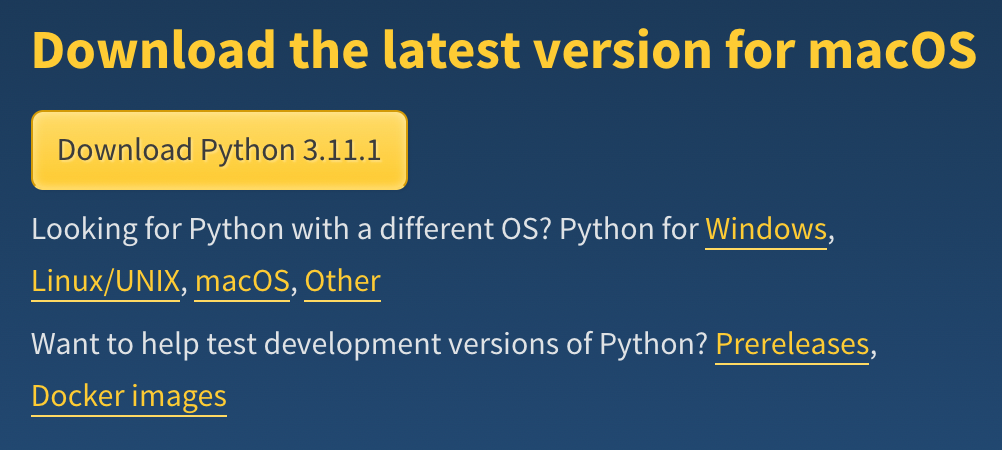
\includegraphics[scale=0.5]{images/download-python.png}}
\caption{Download Python}
\end{figure}
Game chạy tốt nhất với phiên bản 3.6.3 nên nếu gặp vấn đề gì khi chơi với Python bản mới nhất thì nên cài đặt bản 3.6.3 có thể tìm thấy trong cùng đường dẫn trên.
\begin{figure}[H]
\centering{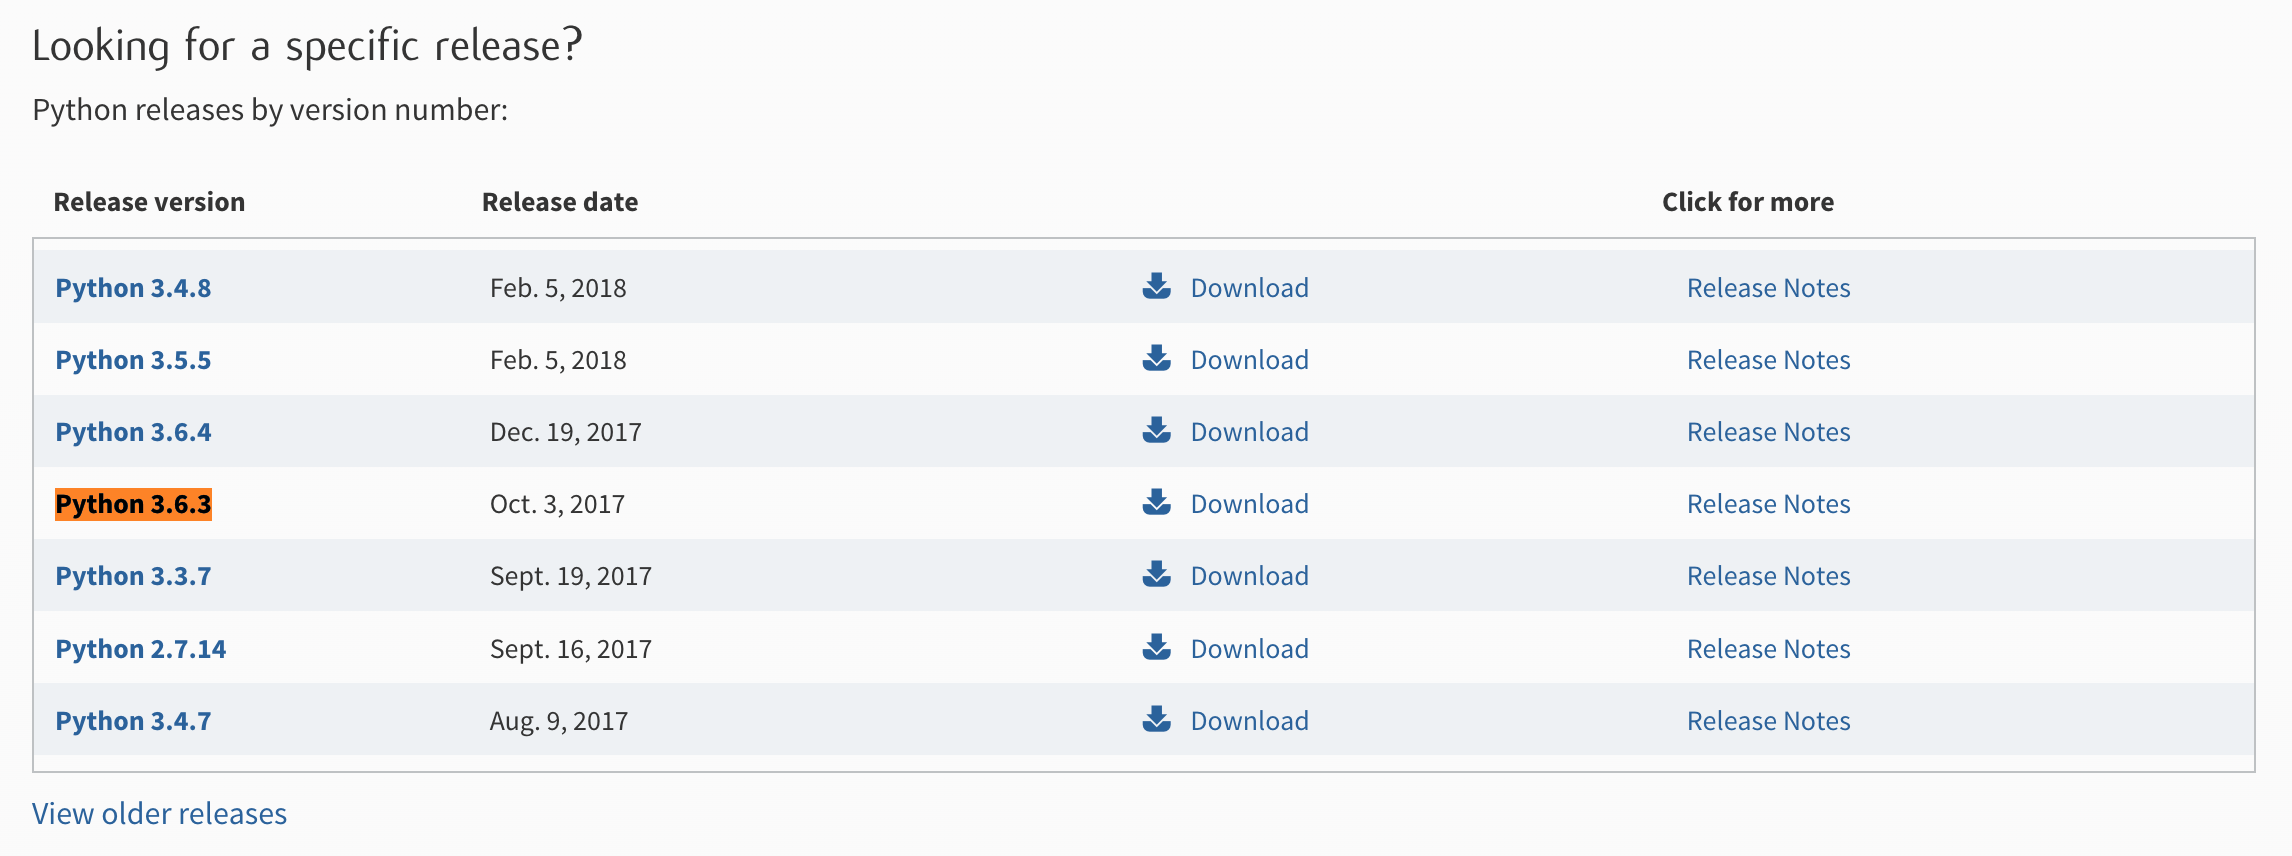
\includegraphics[scale=0.4]{images/python-version.png}}
\caption{Python 3.6.3}
\end{figure}
Sau khi download file cài đặt, ta tiến hành mở file để cài đặt.
\begin{figure}[H]
\centering{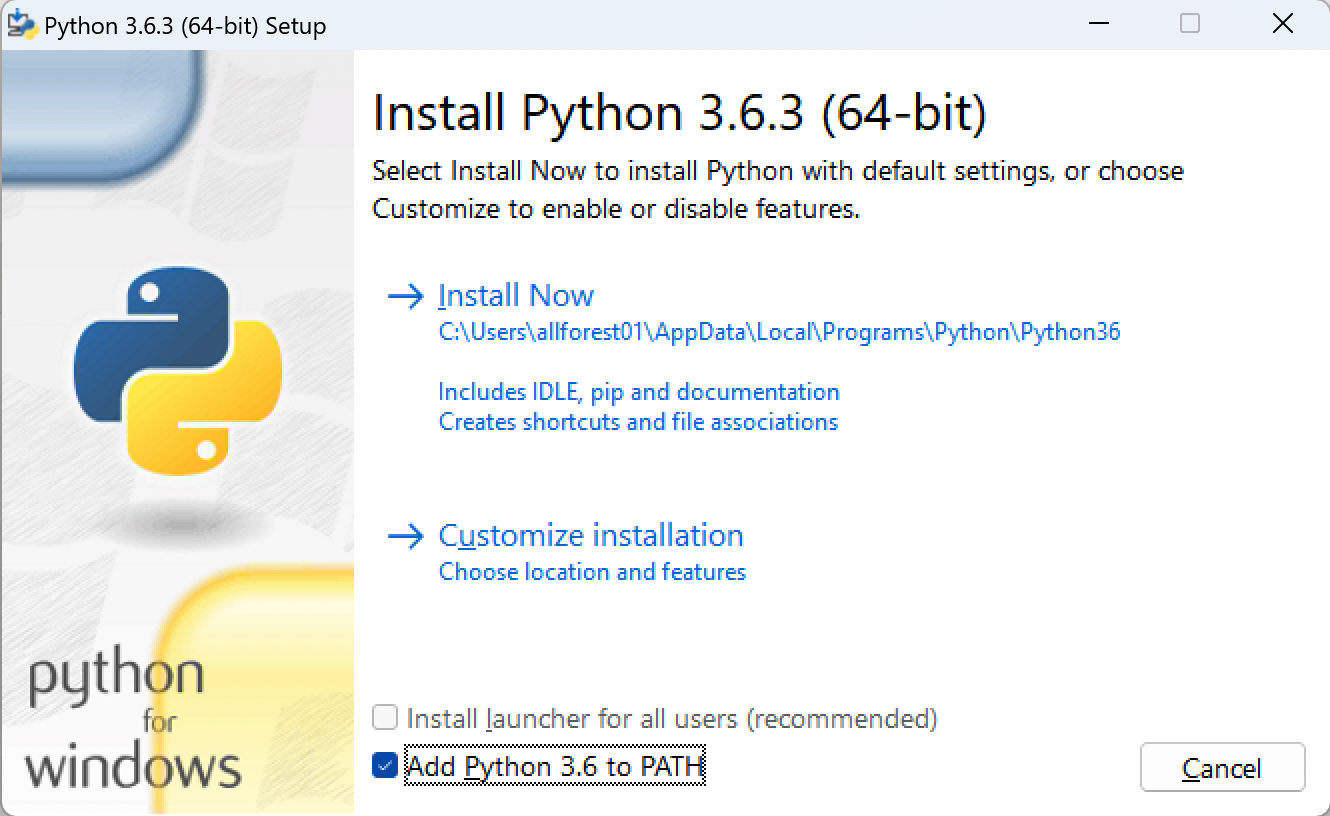
\includegraphics[scale=0.4]{images/setup-python.png}}
\caption{Cài đặt Python}
\end{figure}
Lưu ý cần đánh dấu vào \textbf{Add Python ... to PATH} để việc cài đặt sau này được dễ dàng và thuận tiện hơn. Sau đó nhấn vào \textbf{Install Now} để bắt đầu quá trình cài đặt. Nếu quá trình cài đặt không gặp vấn đề gì thì sẽ hiện cửa sổ thông báo thành công như sau.
\begin{figure}[H]
\centering{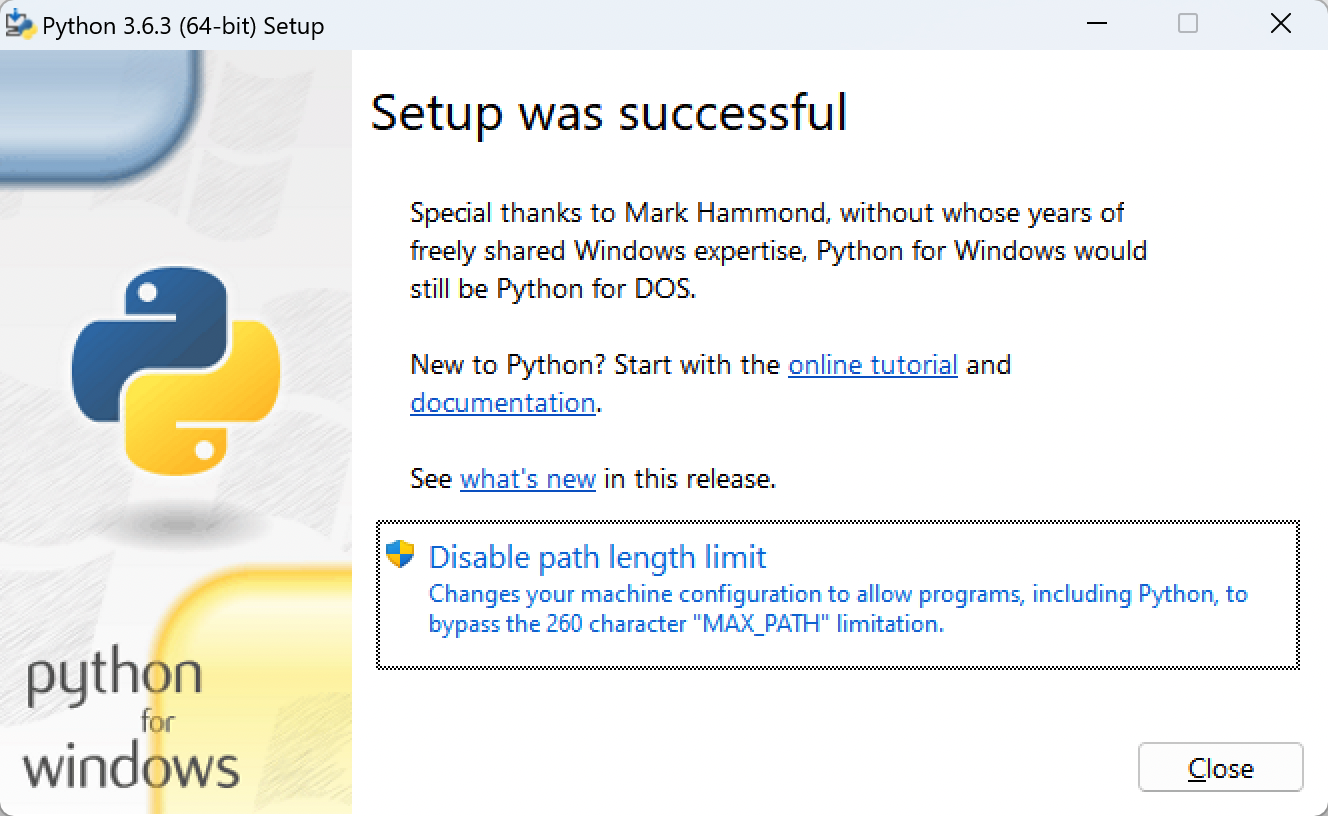
\includegraphics[scale=0.4]{images/setup-successful.png}}
\caption{Cài đặt thành công}
\end{figure}
Sau khi cài đặy Python thành công, ta tiến hành tải source code của game thông qua đường dẫn sau \url{https://github.com/tachithanhdanh/mah-caro-game/archive/refs/heads/main.zip}.
Giải nén main.zip ta có toàn bộ source code của game trong thư mục \textbf{source-code}. Gõ cmd ở đường dẫn của thư mục và nhấn \textbf{Enter} để mở cửa sổ \textbf{cmd} với thư mục hiện tại.
\begin{figure}[H]
\centering{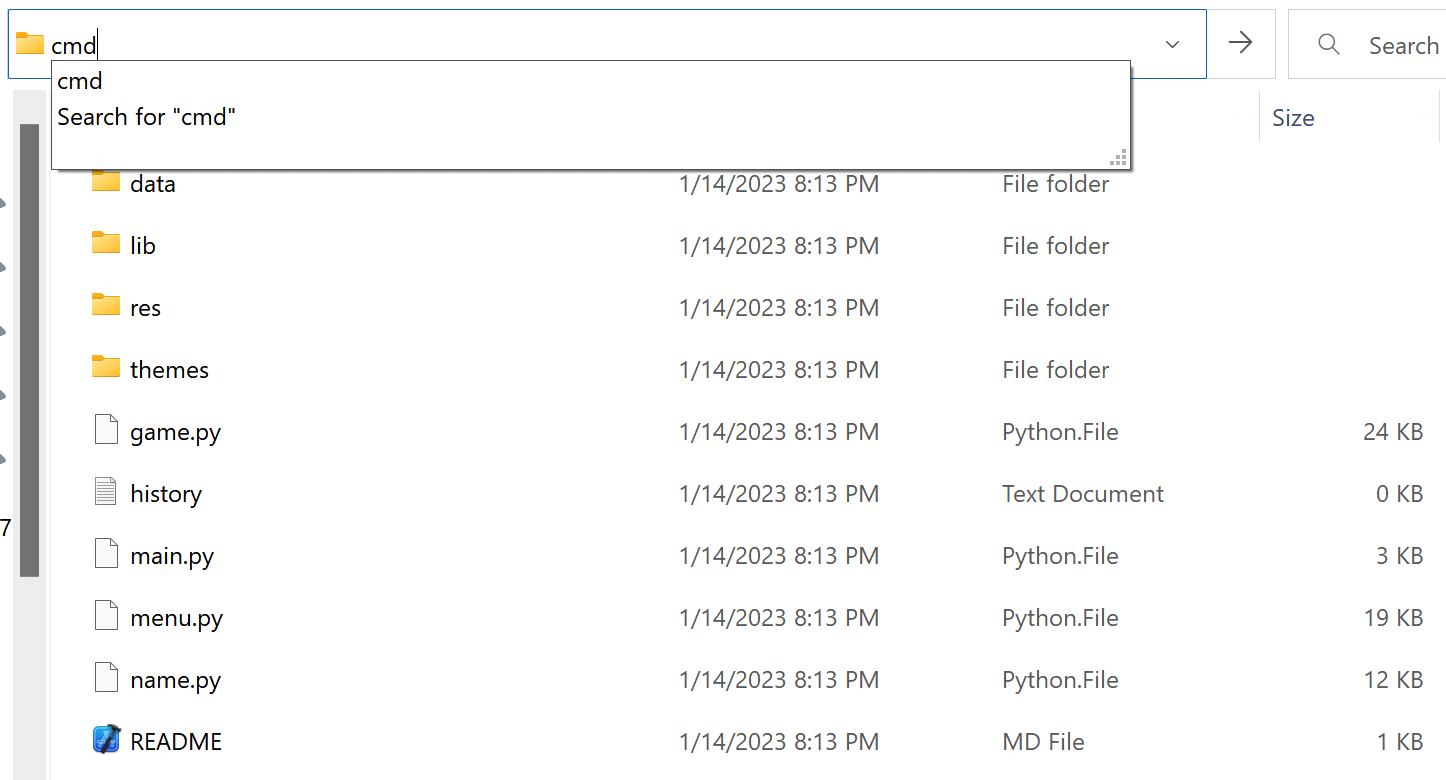
\includegraphics[scale=0.4]{images/source-code.png}}
\caption{Thư mục source-code}
\end{figure}
Lần lượt nhập các lệnh sau để cài đặt các thư viện cần thiết cho việc chạy game:
\begin{lstlisting}https://www.overleaf.com/project/63c3a1b0d79b43b0c5a021fb
pip install pygame
pip install pygame_gui
pip install json
\end{lstlisting}
Cuối cùng ta thực hiện lệnh sau để chạy chương trình:
\begin{lstlisting}https://www.overleaf.com/project/63c3a1b0d79b43b0c5a021fb
python main.py
\end{lstlisting}